



\chapter{Theoretical background}

\section{Entropy}

The entropy of a random variable is a function that describes the ''unpredictability'' of the random variable. In information theory, entropy is the average amount of information contained in each piece of information received, also known as information entropy. \cite{shannon1948mathematical,PATHRIA201139}
\\ \hspace*{\fill} \\
 The information entropy formula given by Shannon \cite{shannon1948mathematical} , for random variable X, is defined as follows, in bits: \\
\begin{equation}
H(X) = - \sum_{i=1}^{n}p(x_{i}) log(p(x_{i}) )  
\end{equation} 
where $p(x_{i})$ represents the probability of the random variable $x$.
\\ \hspace*{\fill} \\
How much information one has needs to be measured by the amount of information. The amount of information received is related to the specific events that occurred. Therefore, the quantity of information is related to the probability of a random event. The smaller the probability of something happening, the greater the quantity of information generated, for example, an earthquake in one part of the earth; the greater the probability of something happening, the smaller the quantity of information generated, for example, the sun rises in the east every day.
\\ \hspace*{\fill} \\
While the information measure is the information brought about by a specific event that has occurred, the entropy is the expectation of the amount of information that possibly generated before the outcome - considering all possible values of that random variable, i.e., the expectation of the amount of information brought about by all possible events.
\\ \hspace*{\fill} \\
The joint entropy measures the uncertainty associated with a set of variables. The joint entropy of two random $X$ and $Y$ variables is defined as: \cite{cover1999elements}
\begin{equation}
H(X,Y) = - \sum_{x}\sum_{y}p(x,y)\log_{2}{p(x,y)}   
\end{equation} 
 Also, the joint entropy satisfies symmetry, i.e. $H(X,Y) = H(Y,X)$ .\\
 
 The conditional entropy quantifies the amount of information needed to describe the outcome of a random variable Y, given that the value of another random variable X is known. The entropy of Y conditioned on X is defined as:
 

\begin{equation}
\begin{split}
H(Y|X) &= \sum_{x\in \mathcal{X}}p(x)H(Y|X = x) \\
&= -\sum_{x\in \mathcal{X}}p(x)\sum_{y\in \mathcal{Y}}p(x,y)\log_{}{p(y|x)} \\
&= -\sum_{x\in \mathcal{X}}\sum_{y\in \mathcal{Y}}p(x,y)\log_{}{p(y|x)}   \\
&= -\sum_{x\in \mathcal{X},y\in \mathcal{Y}}p(x,y)\log_{}{p(y|x)}  \\ 
&= E_{p(x,y)}\left [ -\log_{2}{p(y|x)}  \right ]  
\end{split}
\end{equation}

The Bayesian rule for conditional entropy is expressed as:
\begin{equation}
H(Y|X) = H(X|Y) - H(X) + H(Y)
\end{equation}

\section{Mutual Information}
Suppose there exists a random variable X , and another random variable Y , then their mutual information is defined as : \cite{cover1999elements}
\begin{equation}
I(X;Y) = \sum_{x,y}p(x,y)\log{\frac{p(x,y)}{p(x)p(y)} }  = H(X) - H(X\mid Y)
\end{equation} 
Similarly, the MI between two continuous random variable X and Y is defined as : 
\begin{equation}
I(X;Y) = \iint_{x,y}p(x,y)\log{\frac{p(x,y)}{p(x)p(y)} } = H(X) - H(X\mid Y) 
\end{equation} 
\\ \hspace*{\fill} \\
,where $p(x,y)$ is the joint probability density and, 
\begin{equation}
p(x) = \int \mathrm{d}yp(x,y) \quad and \quad p(y) = \int \mathrm{d}xp(x,y)
\end{equation} 
are the marginals. \cite{carrara2020estimation}
\\ \hspace*{\fill} \\
In 1948, Shannon defined and analyzed this metric, and later Mutual Information was created by Robert Fano \cite{1057418}. MI also affects the difference between the joint distribution of random variables $(X, Y)$ and the product of the bounded distributions of $X$ and $Y$, as we can find from equations (2.3) and (2.4). MI measures the amount of information obtained about one random variable through observing the other random variable. MI can represent a higher-order relationship among variables.\\
At the same time, mutual information can be equivalently expressed as: \cite{mackay2003information}
\begin{equation}
\begin{split}
I(X;Y) &= H(X) - H(X|Y) \\
&=H(Y) - H(Y|X) \\
&=H(X) + H(Y) - H(X,Y) \\
&=H(X,Y) - H(X|Y) - H(Y|X) \\
\end{split}
\end{equation}
The relationship between mutual information and information entropy is shown in the following figure:
\begin{figure}[htbp]
    \centering
    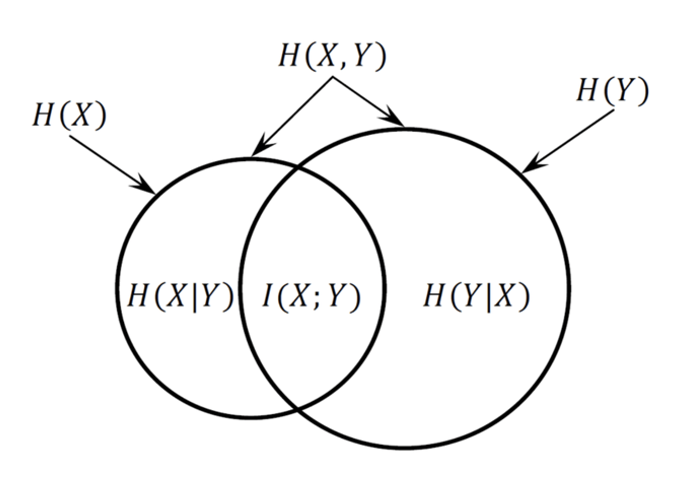
\includegraphics[width=9cm]{report/pics/MI.png}
    \caption{The relationship between mutual information and information entropy}
    \label{fig:my_label}
\end{figure}\\
The figure shows that the two independent variables $X$ and $Y$ are independent when the mutual information $I (X, Y)$ is equal to zero. Also, the mutual information $I (X, Y)$ must be greater than or equal to $I_{min} = 0 $.


\section{Loss of information}
From the theory of mutual information, we know that as $X$ and $Y$ become more correlated, the value of mutual information will become more prominent. A $X$ and $Y$ tend to be independent. The mutual information will become smaller. Therefore, we conjecture that the difference in mutual information will be the amount of information loss concerning information loss. We define information loss as:
\begin{equation}
Loss = I(X;Y) - I(X';Y)
\end{equation}
Under the condition that the mutual information satisfies the symmetry, we take equation (3.8) into (3.9) and get
\begin{equation}
\begin{split}
Loss &= I(X;Y) - I(X';Y)\\
&= I(Y;X) - I(X';Y)\\
&=H(Y) - H(Y|X) - H(Y) + H(Y|X')\\
&=H(Y|X') - H(Y|X)
\end{split}
\end{equation}
\\ \hspace*{\fill} \\
The simplification gives us equation (3.9) which shows that the information loss we calculate equals the difference in conditional entropy for different X and X' relative to Y. The simplified formula avoids the need to calculate other entropy values, thus making it easier for us to work.


\section{Monte Carlo method}
 The Monte Carlo method, also known as the statistical simulation method, is a numerical calculation method guided by statistical probability theory due to the development of science and technology and the invention of electronic computers in the mid-1940s. The Monte Carlo method uses computer-generated samples of a given probability distribution to produce plug-in estimates of specific characteristics of the given distribution. \cite{anderson1986scientific,binder1993monte} \\
\subsection{Monte Carlo approximation}
Suppose X is a random variable with a distribution function $F_{X}(x)$ and suppose that we can generate (through a computer) a sample: \cite{MonteCarlo}
\begin{equation} \nonumber 
\xi _{n} = \left [ x_{1} \dots x_{n}  \right ]  
\end{equation}
of realizations of  n random variables  $X_{1}, ..., X_{n}$ all having distribution function  $F_{X}$. \\

Denote by $F_{n}(x)$ the empirical distribution of the sample $\xi _{n} $ (i.e.,a probability distribution that assigns probability $\frac{1}{n}$ to each one of the values $x_{1}, ..., x_{n}$ .)
Then, the plug-in estimate is a Monte Carlo approximation : 
\begin{equation} \nonumber 
T(F_{n} )  
\end{equation}

\subsection{Monte Carlo integration}
We can approximate an expectation using Monte Carlo integration, which consists of the average of a random sample of observations drawn from the distribution of X to approximate the expectation of the random variable X:  \cite{MonteCarlo}
\begin{equation} \nonumber 
E\left [  X \right ] =\simeq \frac{1}{n}\sum_{i=1}^{n}x_{i}   
\end{equation}
This approximation method is called Monte Carlo integration because the expected value being approximated is in fact an integral:
\begin{equation} \nonumber 
E\left [  X \right ] = \int_{-\infty }^{\infty}x\mathrm{d}F_{X}(x)   
\end{equation}
where $F_{X}(x)$ is the distribution function of $\mathcal{X}$.
Moreover, if  X is a continuous variable, the integral can be written as an ordinary Riemann integral:
\begin{equation} \nonumber 
E\left [ X \right ] = \int_{-\infty }^{\infty } x f_{X}(x)\mathrm{d}x  
\end{equation}
where $f_{X}(x)$ is the probability density function of $\mathcal{X}$.